\section{Preliminaries}
\label{sec:problem}

We consider reasoning problems of the form
$
  \mathcal{T} = (x, V),
$
where $x$ is a problem description (e.g.\ a math question) and
$V(x,y) \in [0,1]$ is a \emph{verifier} that
assigns a score measuring how well a trajectory $y$
solves the problem $x$.

Given a policy $\pi_\theta(\cdot\mid x)$ (e.g.\ an LLM that generates reasoning traces, or an agent that interacts with an environment through a sequence of actions), our goal is to produce a terminal response $y$ that maximizes the verifier score. Let
$\mathcal{Y}_{\mathrm{term}}(x)$ denote the set of valid terminal responses
under the task specification and resource budget. We write the target as
\begin{equation}
  y^{\star}(x) \;\in\; \operatorname*{arg\,max}_{y\in\mathcal{Y}_{\mathrm{term}}(x)}
                       V(x, y).
  \label{eq:obj}
\end{equation}
Finding $y^{\star}$ is important in both training and inference. During
training, high-quality candidates can facilitate post-training or
iterative self-improvement. During inference, $y^{\star}$ is the response
we seek.

The challenge is that the maximization in Eq.~\eqref{eq:obj} is intractable:
on hard problems, the probability mass that $\pi_\theta$ assigns to correct
trajectories can be extremely small. Practical algorithms therefore
approximate $y^{\star}$ by searching over a set of candidates. We 
introduce two common methods below.

\textbf{Best-of-$N$ sampling.}
The simplest approach is to draw $N$ independent trajectories and return the one with the highest verifier score. Formally, let $y^{(1)}, \dots, y^{(N)} \overset{\text{i.i.d.}}{\sim} \pi_\theta(\cdot \mid x)$. The method returns $ y^{\mathrm{BoN}} \;=\; \operatorname*{arg\,max}_{y \in \{y^{(1)}, \dots, y^{(N)}\}} V(x, y) $.
Best-of-$N$ is parallel and requires no structural knowledge of the problem. Its effectiveness, however, is bounded by the finite-sample coverage of $\pi_\theta$: all $N$ trajectories are drawn from the same distribution, so if the optimal trajectory lies in a region with very small policy mass, increasing $N$ gives only linear coverage improvement.

\textbf{Tree search.}
Tree-search methods exploit the sequential structure of a trajectory. A trajectory
is decomposed into steps (e.g.\ tokens, reasoning segments, or agent actions), and the
search maintains a tree whose nodes are partial trajectories and whose edges
correspond to appending a step. Branches are selected and extended according
to a heuristic value so that compute is concentrated on prefixes that look
promising. Classic methods include beam search, best-first search, and Monte
Carlo Tree Search~\citep{mcts}; recent work applies these ideas to LLM and agent reasoning~\citep{tot,treegrpo}. Tree search can be more sample-efficient than best-of-$N$
when the per-step signal is informative, but it still materializes terminal
candidates one lineage at a time through sequential extension.



\section{\ours: Bidirectional Evolutionary Search}
\label{sec:method}

 \ours\ performs a bidirectional evolutionary search that alternates
between two coupled processes: a \emph{forward} search that seeks
better candidates, and a \emph{backward} search that decomposes
the problem into fine-grained sub-goals to evaluate each forward
node. The forward search not only extends trajectories but also
recombines parts of different candidates, producing solutions that
no single rollout from $\pi_\theta$ would likely reach. The backward
search provides dense and interpretable scores for partial
trajectories, guiding the forward search toward promising
candidates. In practice, one backward search step is performed after every
several forward search steps. The full pseudocode is given in
Appendix~\ref{app:algo}, and a case study illustrating the search
process is provided in Appendix~\ref{app:case}.

\subsection{Forward Search: Expanding the Reachable Solution Space}
\label{sec:forward}

\begin{figure}[t]
\centering
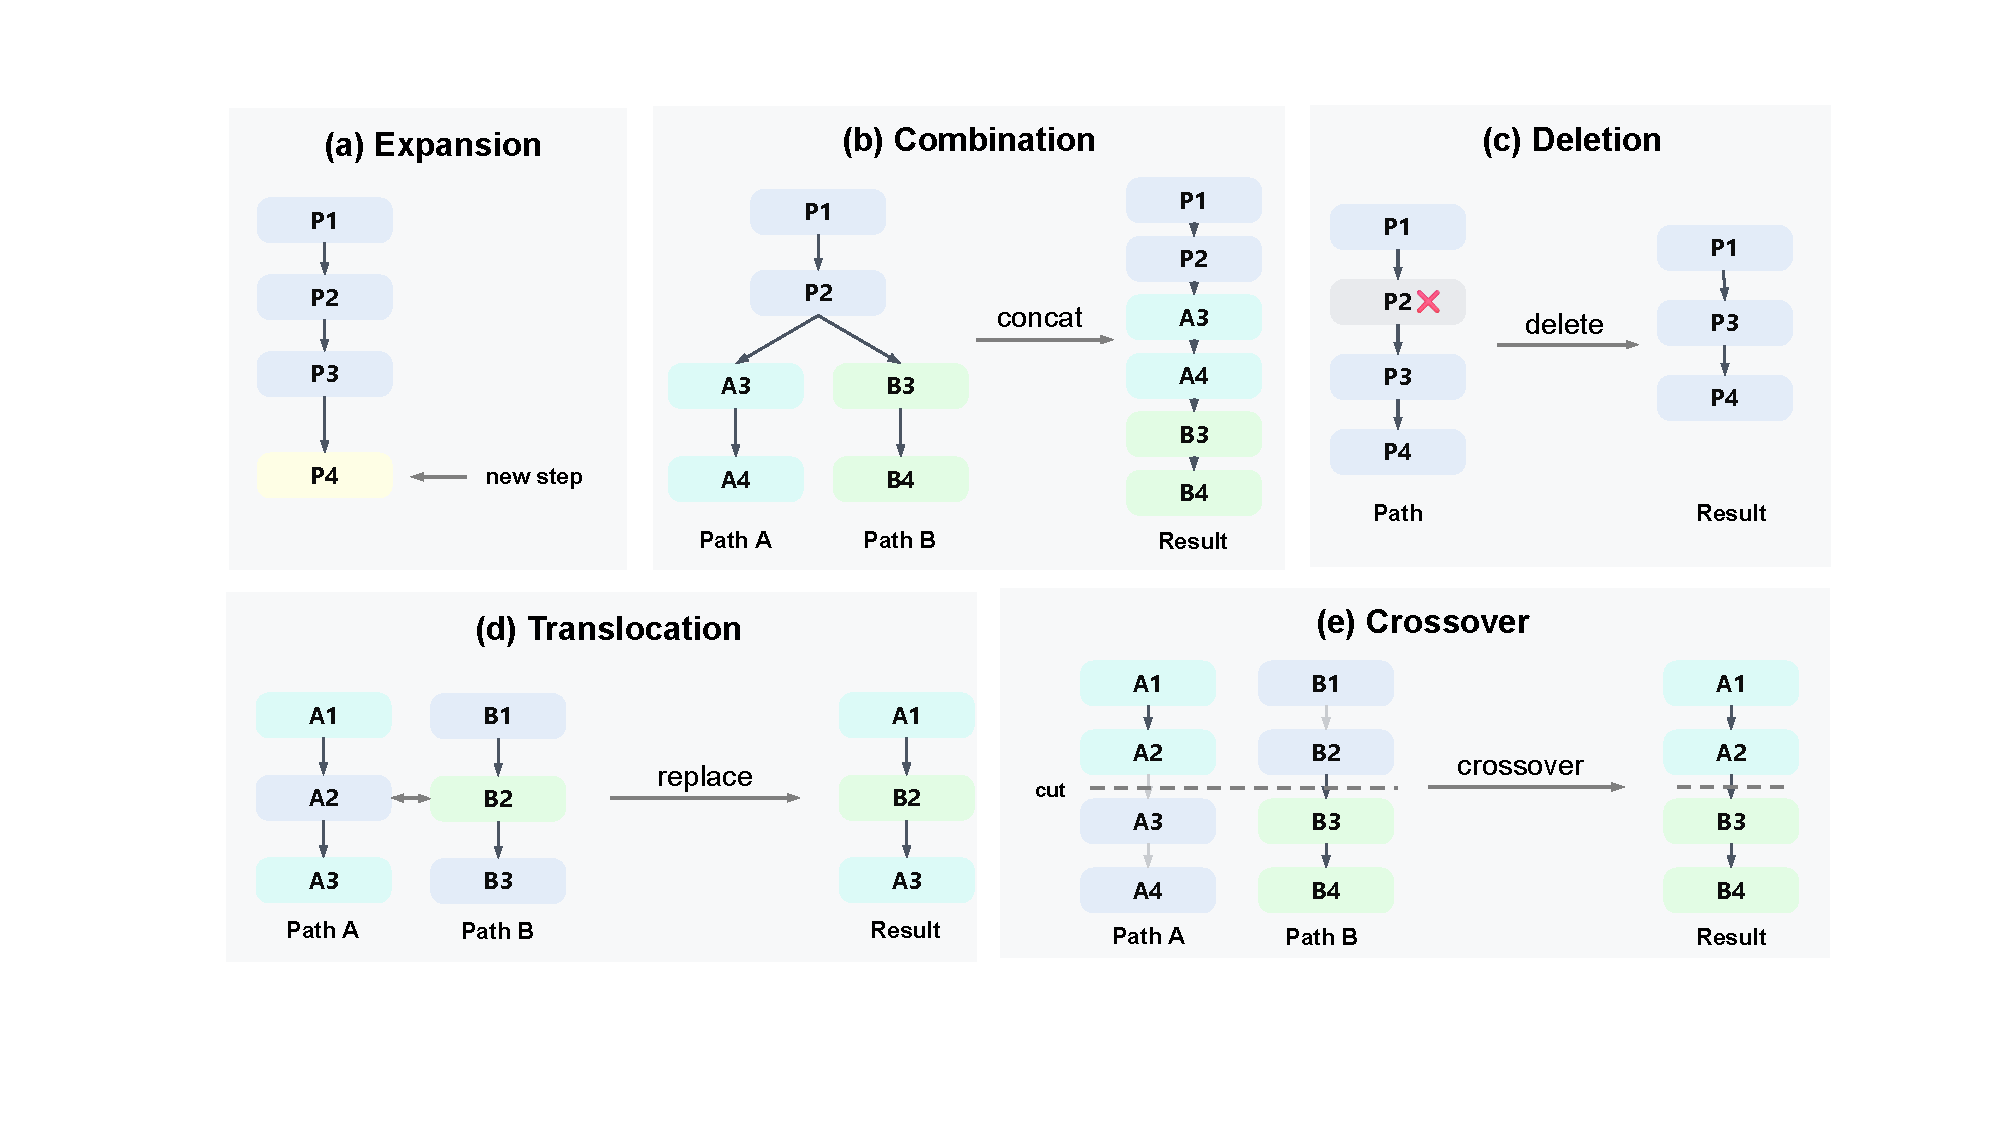
\includegraphics[width=\linewidth]{images/forward.pdf}
\caption{Forward search operators. \textbf{(a) Expansion:} the policy generates new steps (yellow). \textbf{(b) Combination:} two trajectories sharing a common prefix (P1--P2) have their distinct suffixes concatenated into a single candidate. \textbf{(c) Deletion:} an interior step (P2) is removed. \textbf{(d) Translocation:} one step in Path A (A2) is replaced by a step from Path B (B2). \textbf{(e) Crossover:} Path A is cut at a splice point and its tail is replaced by the tail of Path B. }
\vspace{-1em}
\label{fig:forward}
\end{figure}

We represent each candidate partial trajectory as a node
$n=(y_1,\dots,y_{t})$, where $y_i$ denotes the $i$-th step (e.g.\ a reasoning segment or an action). The search maintains a candidate set $\mathcal{P}$ of such nodes, and at
each search step applies one of two types of operators, \emph{expansion}
or \emph{evolution}, to produce a child node $n'$, which is scored by
the backward search (Section~\ref{sec:backward}) and added to $\mathcal{P}$.


\textbf{Expansion.}
Expansion extends a parent node by sampling new steps. Given
$n=(y_1,\dots,y_{t})$, we sample a step count
$K\sim\mathrm{Uniform}\{1,\dots,K_{\max}\}$ and draw up to $K$ new steps from
$\pi_\theta$:
\begin{equation}
  y_{t+k}\,\sim\,\pi_\theta\bigl(\cdot\mid x\oplus y_1\oplus\cdots\oplus y_{t+k-1}\bigr),
  \qquad k=1,\dots,K,
  \label{eq:expand}
\end{equation}

\textbf{Evolution.} 
 A key limitation of expansion alone is that each candidate
is built by sequentially extending a single trajectory,
so it cannot combine useful parts from different candidates.
Evolution operators overcome this by editing and recombining
existing trajectories. As illustrated in Figure~\ref{fig:forward}, we define four operators inspired by biological evolution: \textit{(i) Combination} merges two trajectories by concatenating their suffixes beyond a shared prefix; \textit{(ii) Deletion} removes one interior step, producing a shorter candidate; \textit{(iii) Translocation} transplants a single step from one trajectory into another; and \textit{(iv) Crossover} splices the prefix of one trajectory onto the tail of another. Formal definitions are provided in Appendix~\ref{app:operators}. 
Together, these four evolution operators allow the search to restructure, condense, and recombine existing trajectories. As with mutations in nature, evolution operations are not guaranteed to produce better candidates. However, the value of evolution lies in generating diverse candidates: \textbf{\textit{even if only a small fraction turn out to be improvements, that is sufficient for the search to make progress.}}
Here, the four evolution operators are defined as direct edits on the step sequence. In settings where direct concatenation is not well-defined, the evolution operators can alternatively be implemented by prompting the policy model.


At each forward search step, we select among the operators with fixed
probabilities. All operators require selecting one or two parent nodes from
$\mathcal{P}$. Let $\mathcal{C}_t$ be the set of eligible non-terminal members of
$\mathcal{P}$ at step $t$. For single-parent operators (expansion, deletion), we sample the parent from a Boltzmann distribution over backward score $s(n)$ (Eq.~\ref{eq:score}):
\begin{equation}
  \Pr\bigl[n\mid\mathcal{C}_t\bigr]
    \;=\;\frac{\exp(\tilde{s}(n)/\tau_t)}
              {\sum_{n'\in\mathcal{C}_t}\exp(\tilde{s}(n')/\tau_t)},
  \qquad
  \tilde{s}(n) \;=\; s(n) + \lambda\cdot\mathbf{1}\!\bigl[\deg(n)=0\bigr],
  \label{eq:boltz}
\end{equation}
where $\tau_t>0$, $\deg(n)$ is the number of children of $n$ in
$\mathcal{P}$, and the indicator term adds a small constant bonus
$\lambda$ (we use $\lambda=0.1$) to candidates that have not yet been
selected as parents, giving unexplored nodes a higher chance of being expanded.

For two-parent operators (combination, translocation, crossover), we select a pair of parent nodes $(n_a, n_b)$ from $\mathcal{C}_t$.
We calculate a pair score $s(n_a, n_b)$ (Eq.~\ref{eq:pair_score}) that favors complementary parents whose strengths cover different parts of the problem.
The pair is then drawn from the analogous Boltzmann distribution:
\begin{equation}
  \Pr[(n_a, n_b) \mid \mathcal{C}_t]
   \;=\;\frac{\exp(s(n_a, n_b)/\tau_t)}
              {\sum_{n_a, n_b\in\mathcal{C}_t}\exp(s(n_a, n_b)/\tau_t)}.
        \label{eq:bi_boltz}
\end{equation}
The temperature $\tau_t$ is annealed linearly from an initial value
$\tau_0$ to a final value $\tau_{\mathrm{end}}<\tau_0$ over the search
budget, gradually shifting from exploration to exploitation.

\subsection{Backward Search: Better Verification through Goal Decomposition}
\label{sec:backward}

While the verifier $V$ provides a score for each node in the forward search, this signal is relatively sparse. Backward search addresses this by decomposing
the problem into a tree of fine-grained sub-goals. Each forward
node is then scored against this tree: the more sub-goals a
candidate trajectory has addressed, the higher its score.
This gives the forward search a dense, informative signal to
select promising candidates, even when none of them have fully
solved the problem yet. 

Below we describe how the backward search is constructed.
Starting from the top-level goal $g_{\texttt{root}}$ (i.e.\ solving the
entire problem), the policy $\pi_\theta$ is prompted
to break each goal into finer sub-goals, producing a rooted backward goal tree. Each goal $g$ on the tree can be recursively split into children
$\mathrm{ch}(g)$ (finer sub-goals), and every $g$ comes with a verifier
$V_g(x,n) \in [0,1]$ that tests
how well a candidate node $n$ addresses the sub-goal $g$ on
problem $x$. For the top-level goal, $V_{g_{\texttt{root}}} = V$ (the verifier of the original problem). 
This decomposition is re-invoked every $K$ forward
search steps: at each invocation, we select a leaf sub-goal that no current candidate fully satisfies and prompt $\pi_\theta$ to split it into finer sub-goals. After that, all existing forward nodes are re-scored. 
The verifiers are task-dependent and can be instantiated
as rule-based checkers, test-case code executors, embedding similarity
models, or LLM judgers. We describe the verifiers used in each experiment
in Appendix~\ref{app:setup}.


For example, consider the problem ``Compute
$\frac{(4+6)\times 3}{2} - 5$.'' The backward search
can produce the following goal tree:

\begin{center}
\begin{forest}
  for tree={
    grow'=0,
    anchor=west,
    child anchor=west,
    parent anchor=east,
    l sep=12mm,
    s sep=4mm,
    edge={->,>=latex},
    font=\small,
  }
  [$g_{\texttt{root}}$: compute $\frac{(4+6)\times 3}{2} - 5$
    [$g_1$: compute $(4+6)\times 3$
      [$g_{1.1}$: compute $4+6$]
      [$g_{1.2}$: \#1 multiply by $3$]
    ]
    [$g_2$: \#1 divide by $2$]
    [$g_3$: \#2 subtract $5$]
  ]
\end{forest}
\end{center}

For a candidate node $n$ from the forward search
(Section~\ref{sec:forward}) and a sub-goal $g$, define the
sub-goal score
\begin{equation}
  s(n,g) \;=\; \alpha\cdot V_g(x,n)
    \;+\;(1-\alpha)\cdot\frac{1}{|\mathrm{ch}(g)|}
    \sum_{g'\in\mathrm{ch}(g)} s(n,g'),
  \label{eq:score}
\end{equation}
where $\alpha\in[0,1]$ balances the contribution of coarser parent goals and
finer-grained sub-goals to the overall score. For leaf sub-goals ($\mathrm{ch}(g)=\emptyset$),
we set $s(n,g)=V_g(x,n)$. If a goal is already fully
satisfied ($V_g(x,n)=1$), we short-circuit to $s(n,g)=1$ without
evaluating its children. 
The overall score is $s(n)\triangleq s(n,g_{\texttt{root}})$.

For two candidate nodes $n_a$ and $n_b$, we further define a pair score that measures their joint coverage of the goal tree.
Replacing each sub-goal verifier with the maximum of the two
parents' scores gives
\begin{equation}
  s(n_a,n_b,g) \;=\; \alpha\cdot \max\{V_g(x,n_a),\, V_g(x,n_b)\}
    \;+\;(1-\alpha)\cdot\frac{1}{|\mathrm{ch}(g)|}
    \sum_{g'\in\mathrm{ch}(g)} s(n_a,n_b,g'),
  \label{eq:pair_score}
\end{equation}
with $s(n_a,n_b)\triangleq s(n_a,n_b,g_{\texttt{root}})$. A sub-goal is
considered covered if either parent addresses it, so the pair
score favors complementary parents that cover different parts
of the goal tree.

Applying this procedure to every node in the forward search
tree yields a backward score for each node and a pair
score for each pair of nodes, which directly drive node
selection in the forward search.

\subsection{Using \ours\ for Post-Training and Inference}
\label{sec:usage}

\textbf{Post-Training.}
\ours\ replaces the sample-generation stage of post-training. Given a training problem, \ours\ returns a set of high-quality trajectories from the forward search candidate set $\mathcal{P}$. These trajectories are then used as training data for post-training algorithms, replacing the candidates that would otherwise be obtained from i.i.d.\ rollouts.
Because \ours\ can find correct solutions that single rollouts
rarely reach, it provides stronger training signal, especially
on hard problems.

\textbf{Inference.}
At inference time, \ours\ runs on open problems with a
fixed compute budget, and the terminal trajectory with the
highest score is returned as the final answer. 